\documentclass[conference,a4paper]{IEEEtran}

% Escritura mejorada de fórmulas matemáticas
\usepackage{amsmath}
% Inserción de gráficos
\usepackage{graphicx}
\graphicspath{ {images/} }
% Escritura de pseudocódigo
\usepackage[kw]{pseudo}
\usepackage{algorithm}
\usepackage[noend]{algpseudocode}
% Escritura mejorada de tablas
\usepackage{booktabs}
% Escritura mejorada de citas bibliográficas
\usepackage{cite}
% Hipervínculos
\usepackage{hyperref}
\hypersetup{
    colorlinks=true,
    linkcolor=blue,
    filecolor=magenta,      
    urlcolor=cyan,
}
\urlstyle{same}

% Macros traducidas
\def\contentsname{Índice general}
\def\listfigurename{Índice de figuras}
\def\listtablename{Índice de tablas}
\def\refname{Referencias}
\def\indexname{Índice alfabético}
\def\figurename{Fig.}
\def\tablename{TABLA}
\def\partname{Parte}
\def\appendixname{Apéndice}
\def\abstractname{Resumen}
% IEEE specific names
\def\IEEEkeywordsname{Palabras clave}
\def\IEEEproofname{Demostración}

%Título
\title{Clustering con Incertidumbre}

%Autores
\author
{
	\IEEEauthorblockN{Víctor Muñoz Ramírez}
	\IEEEauthorblockA
	{
		\textit{Dpto. Ciencias de la Computación e Inteligencia Artificial}\\
		\textit{Universidad de Sevilla}\\
		Sevilla, España\\
		vicmunram@us.es
	}
	\and	
	\IEEEauthorblockN{Enrique Reina Gutiérrez}
	\IEEEauthorblockA
	{
		\textit{Dpto. Ciencias de la Computación e Inteligencia Artificial}\\
		\textit{Universidad de Sevilla}\\
		Sevilla, España\\
		enrreigut@us.es
	}
}

\begin{document}
\maketitle

%Investigación Kike

\section{Investigación Kike}

Según la  \hyperref[bib:georgeSeif]{Referencia 1}: \\ 

Empieza con una pequeña introducción respecto a  lo que que es Clustering en Machine Learning. Una técninca para poder separar un conjunto de puntos dados. Estos puntos deben de poseer algún tipo de caracteristica común que nos permita poder indentificar unos de otros y así poder agruparlos.\\

Habla de 5 técnicas de algoritmos de Clustering: K-Means, Mean-Shift, Density-Bases Spatial con Ruido, Expectation-Maximization (EM) usando mezcla de modelos Gaussianos (GMM) y Agglomerative Hierarchical Clustering. Cada uno presenta sus ventajas y desventajas, que ire desarollando a lo largo de los siguientes puntos:\\

K-Means:\\

Este es el algoritmo que es presentado en las transparecias de teoría. Según el artículo es uno de los métodos mas fácil de implementar y de entender.  Lo primordialment destacable es que el input inicial es tuyo, es decir, debes primero observar los datos y tratar de indentificar el posible número o cantidad  de grupos(clústeres) que puedes identificar según las densidades de los puntos.\\

Este algorimos consiste, en como ya se menciono anterioirmente, seleccionar tantos puntos considerados como centros de los clusters que considermaos que hay según lla representación dimensional de los datos. El algoritmo es iterativo, es decir, con cada iteración los centros se van desplazando de forma que se sitúen en el centro de cada clúster. Esto se consigue midiendo la distancia de los puntos con cada centro para ver a cual corresponden.\\

La ventaja de este método es que un algoritmo que es considerado bastante rápido con un complejidad de $\mathcal{O}(n)$. Sin embargo partes con la premisa de que debes seleccionar cuantos grupos de clúster quieres. Esta decisión no siempre es trivial. Una alternativa es realziar aproximaciones como en función de la cantidad de puntos,  introducir \textit{x} centros pero esto puede provocar resultados difrerentes, por ende resutlando en una falta de consistencia.\\

Otra posible optimización de este algoritmo es ahorrarnos el tener que situar los puntos manualmente y simplemente indicar cuantos queremos. Esto suele realizarse mediante la inicialización aleatoria de estos puntos, no obstante, volvemos a encontrarnos con el problemas de la falta de consistencia.\\

La Referencia ofrece una alternativa a K-Means conocida como K-Medians. La principal diferencia es que a la horta de recomputar los centros nos basamos en la mediana y no en la media. Este método es menos sensitivo a valroes atípicos sin emaego es más cosotoso de forma computacional ya que requiere \textit{sorting} para computar la mediana del vector de los datos.\\

Mean-Shift:\\

Este algoritmo es un algoritmo basado en enventanado que trata de encontrar las areas mas densas de puntos con el fin de determinar el centro de los clusters de puntos dados. Este algoritmo es denominado en inglés como \textit{centroid-base algorithym}. Esto nos describe la función de este algoritmo la cual es encontrar el centro de los clusters formado por el conjunto de puntos dados en funcion de la densidad de estos.\\

El funcionamiento de este algoritmo es sencillo. Lo primero que se hacer es inicializar un punto de forma aleatoria en el espacio de puntos con un radio de busqueda. La superficie cubierta por el círculo (ventana circular la cual se le conoce como \textit{kernel}) se encarga de contar los puntos incluidos en este. El vector dirección en el que se mueve se hace en función del centro de masa, es decir, donde se vayan concentrando los puntos.\\

La forma en la que este algoritmo converge, es que en vez de inicializar una única ventana, se inicializan varias distribuidas de forma uniforme por el espacio de puntos. Vamos iterando hasta  que las distancia entre el centro de las ventanas sean cubiertas por todas.\\

La ventanja de este algoritmo respecto a K-Means es que no requerimos de indicar el número de centros que vamos a querer, si no que se detectan solos basados en la desidad de puntos, sin embargo esta ventaja que presenta puede llegar a ser una desventaja. Este método es perfecto para encontrar el centro de los puntos que formen parte de clusters que esten separados y sean densos. En el escenario de que los cluster conformen figuras, tipo el perímetro de un círculo, el algoritmo puede que no agrupe los puntos en único conjunto, sino que haga un subdivisión de estos. Otra desventaja que presenta es que se deben escoger la longitud del radio resultando factor determinista que puede provocar diferentes resultados.\\

Density-Based Spatial Clustering con ruidos (DBSCAN):\\

Este algoritmo también esta basado en la agrupación de los puntos en función de su densidad. La gran diferencia que presenta respecto a Mean-Shift es que no trata de localizar el centro del conjunto de los puntos, si no que va generando a agrupación al vuelo.\\

El funcionamiento del algoritmo es muy simple. Sen encarga de ir recorriendo todos los puntos del conjunto de puntos y mira en un radio alrededor de este. Si se encuentra un punto dentro de este radio, se le asigna como parte del clúster. Los puntos que se leen, se marcan como visitados. En el momento que ha acabdo de "agrupar un conjunto de puntos" pasa al siguiente en la lista de puntos .\\

Este algoritmo presenta ventajas respecto a K-Means ya que como en Mean-Shift no es necesario indicar de antemano el número de agrupaciones que identificamos o vamos a querer, además de  que a difrencia de Mean-Shift es capaz dde identificar figuras. Sin embargo, también tiene su desventaja la cual es que requiere cierta distancia mínima entre los puntos para poder agrupar todo en la misma figura, ya que la distancia a la que miramos, conocida como Epsilon, varía en función de la densidad de puntos en esa zona.\\

El artículo habla de otros dos algoritmos los cuales no consideranmos relevantes para el objetivo que se nos propone pero consideramos que son muy interesantes  y presentan alternativas a la hora de agrupar diferentes grupos de puntos.\\

De momento las técnicas de \textit{clustering} presentadas, como hemos redactado, tienen sus ventajas y desventajas en las cuales nos basaremos para tratar el tema de nuestro objetivo. El principal porblema encontrado es que en función de la distribución de puntos, conviene más una técnica que otra de forma que la dificultad se encuentra en automatizar la clasificación de los puntos de forma que siempre se use la técnica más efectiva para agrupar puntos.\\

Contando con la desventaja presentada anteriormente, igualemente debemos de elaborar un algoritmo que ataje el problema propuesto. Tras la investigación realziada hasta el momento, creemos que DBSCAN es la opción más factible, sin embargo tenemos en  mente el problema de que requiere cierta densidad de puntos que conformen la circunferencia. Por ello, la siguiente idea propuesta es realizar una mezcla entre K-Means y Mean-Shift. El objetivo es inicializar una cierta cantidad de centro de forma que estos cubran todo el espacio de puntos y luego vamos aproximando los centros por iteración como en K-Means. La condición de parada sería cuano estos centros convergan. \\

Creemos que K-Means es la segunda mejor opción ya que el algoritmo como su nombre indica, no esta basado en la debsidad de puntos, sino en la media de la posición de esto. Esto nos interesa ya que las circufenrencias generalmente lo puntos estarán distribuidos de forma que en el centro de esta no exista ningún punto salvo que se colapse con otra circunferencia. Estos caso específicos serán estudiados con mayor precisión en el estudio del problema.\\

\clearpage

%Estructura del proyecto

\section{Estructura del proyecto}

\textbf{\\Dominio del problema y generación de ejemplos}\\

En primer lugar, se implementaron aquellas clases relativas a los elementos del dominio del problema, \textit{Point} y \textit{Circunference}, que sirven para representar el conjunto de puntos de entrada y las resultantes circunferencias que agrupan a estos.
La primera solo almacena las coordenadas x e y de un punto, mientras que la segunda almacena el centro y radio de una circunferencia; además del conjunto de puntos usados para su representación gráfica. Ambas clases, durante el desarrollo del proyecto, fueron aumentando en tamaño al incluirse en ellas métodos necesarios para la implementación del algoritmo.\\

Tras la elaboración de estas clases, se decidió diseñar las necesarias para la generación de ejemplos y representación gráfica de estos mismos. El objetivo era poder comprobar la eficacia de las distintas partes del algoritmo a medida que se desarrollaba con una buena variedad de casos de prueba; pudiéndose encontrar los fallos que podrían haberse cometido y subsanarlos lo antes posible.\\

Estas clases son \textit{DataSet} y  \textit{Canvas}, que nos permiten, respectivamente, realizar la carga de datos de un ejemplo a partir de un archivo .csv y elaborar y representar estos. En cuanto al formato de los archivos .csv, este viene detallado en el archivo README.txt adjunto al código. En cuanto a la generación de ejemplos, se crearon métodos aleatorios para la creación de distribuciones de circunferencias, la eliminación de un porcentaje de puntos y la inserción de ruido desviando estos. Este desvío se hace adaptando el método \textit{numpy.random.normal} el cual proporciona valores aleatorios dentro de una distribución. Para la adaptación solo es necesario aportar la desviación que queremos en dicha distribución.\\
La generación de un nuevo ejemplo consiste en crear una distribución aleatoria, eliminar algunos puntos de ella y desviar los restantes para tener algo de ruido. El único problema de esta forma de actuar, es que si se queremos un ejemplo muy concreto, es necesario crearlo a mano o bien ejecutar el método hasta tener un caso similar al buscado. Como ya se ha mencionado, \textit{Canvas} nos permite también representar dichos ejemplos mostrándonos de forma conjunta los puntos y circunferencias del problema.\\
\newpage
\begin{figure}[h]
\centering
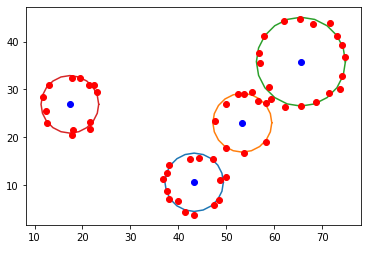
\includegraphics[scale=0.8]{EjemploGenerado}
\caption{Ejemplo generado de forma aleatoria, porcentaje de eliminación=30\%, escala del desvío=0.5}
\end{figure}


A continuación, se realizó la implementación de los objetivos específicos relativos al código siguiendo el orden en el que aparecían en el documento; ya que iban de menos a más en la elaboración del algoritmo final.\\

\textbf{Estructura de datos}\\

De esta manera, se diseñó para almacenar la información de cada iteración del algoritmo una estructura de datos basada en dos arrays: 
\begin{itemize}
	\item Clusters: Almacena objetos de la clase \textit{Circunference}, los cuales representan. El orden de estos en el array viene definido por como se inicializaron.
	\item Threshold: Almacena arrays con los grados de pertenencia de cada punto a cada cluster. El orden de estos viene definido por como estuvieran los puntos ordenados en el archivo .csv.\\
\end{itemize}

\textbf{Cálculo de circunferencias}\\

Tras esto, se elaboró un método para calcular centro y radio de una circunferencia a partir de un listado de puntos.\\ 
La primera versión de este método calculaba el centro como el baricentro del conjunto y el radio como la distancia media de este a todos los puntos. Este método, aunque muy eficiente incluso con ruido, fallaba cuando se le proporcionaba un arco en lugar de una circunferencia; ya que como el baricentro se sitúa en función de la densidad, el centro queda muy cerca del arco resultando en un radio menor al debido, y quedando los puntos de los extremos muy alejados de la circunferencia.\\

\newpage
\begin{figure}[h]
\centering
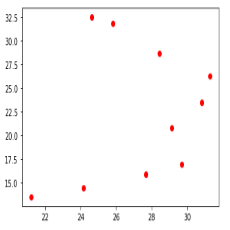
\includegraphics[scale=0.9]{ArcoBaricentro}
\caption{Ejemplo con los puntos en forma de arco}
\end{figure}

\begin{figure}[h]
\centering
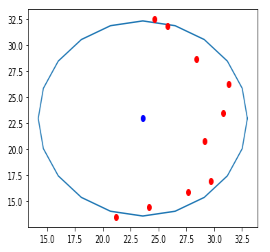
\includegraphics[scale=0.8]{ArcoBaricentroResultado}
\caption{Circunferencia calculada usando el baricentro}
\end{figure}

Por ello, se decidió implementar un segundo método que calculara el centro como el circuncentro del conjunto; ya que con la circunferencia circunscrita nos aseguramos que al menos pase por tres puntos de los proporcionados, y el radio como la distancia desde este a uno de esos puntos. Este se calcula como el punto de corte de las mediatrices de los segmentos que forman los puntos seleccionados, \hyperref[bib:georgeSeif]{Cálculo del circuncentro}. El problema de esta forma de calcularlo es que los puntos elegidos hagan que las mediatrices no se corten y no haya solución, lo cual fue solventado haciendo que el cálculo se repitiera hasta que esta existiera.\\

\newpage
\begin{figure}[h]
\centering
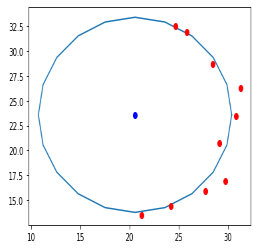
\includegraphics[scale=0.8]{ArcoCircuncentroResultado}
\caption{Circunferencia calculada usando el circuncentro}
\end{figure}

Como vemos, la selección de los puntos es muy importante y ha sido un elemento que se ha tratado de múltiples formas. El planteamiento inicial  consistía en tomar un punto aleatorio, buscar el más lejano a este y por último buscar uno a una distancia intermedia de ambos. Esta forma requería cierto coste computacional adiciona con respecto al baricentro;l ya que había que recorrer el listado de puntos más de una vez, pero reaccionaba bien incluso con arcos. Sin embargo, en situaciones con mucho ruido el resultado se desviaba. Se intentaron otras formas de seleccionar estos puntos, por ejemplo, siguiendo la estructura anterior pero siendo el último punto uno aleatorio también. Sin embargo, ninguna terminaba de funcionar; así que finalmente se optó porque todos fueran aleatorios ya que el resultado era muy similar y requería un coste computacional mucho menor.\\

Finalmente, se dejaron tanto el método que utiliza el baricentro como el que utiliza el circuncentro para poder comprobar con el algoritmo final como reaccionaba cada uno y cual era más eficiente.\\

\textbf{Cálculo de grados de pertenencia}\\

Después, se implementó el método correspondiente al cálculo de los grados de pertenencia.\\
Como primer paso se calculan todas las distancias del punto a los clusters, tras lo cual se realiza un sumatorio de todas ellas. A este se le restan las distancias por separado, para que los grados de pertenencia sean inversamente proporcionales a la distancia. Y para que dichos valores esten normalizados, se dividen los resultados de la operación anterior entre el sumatorio.\\
Cabe destacar que durante la experimentación con el algoritmo final, en ocasiones al intentar normalizar se producían divisiones por cero; lo cual fue solventado instanciando el sumatorio de los puntos con una cantidad despreciable.\\
Posteriormente, se diseñó una modificación de este método que calcula los grados de pertenencia para todos los puntos de un problema, devolviendo el array correspondiente a Threshold, ya mencionado antes. Para esto se llama al método anterior por cada uno de los puntos del problema.\\

\textbf{Implementación del esquema general}\\

Finalmente, se implementó la clase \textit{ClusteringSolver} en la cual encontramos el método \textit{learn}, el cual sigue el esquema general planteado con pequeñas modificaciones que comentaremos más adelante; pero primero vamos a centrarnos en lo que tienen en común ambas.\\

Para la inicialización, desde un inicio se decidió instanciar las circunferencias de forma aleatoria, concretamente, se toma como centro un punto aleatorio del listado y se le proporciona un radio también aleatorio. Además, se decidió permitir al usuario elegir si utilizar baricentro o circuncentro para recalcular las circunferencias. Aunque es cierto, que si el conjunto de puntos suministrado para un cluster es menor de tres, se utiliza el baricentro ya que el circuncentro necesita como minimo esa cantidad.\\

En cuanto al criterio de parada, primero se implementó con un número fijo de iteraciones ya que era más sencillo y permitía comprobar el comportamiento del algoritmo con facilidad; aunque finalmente se acabó implementando un criterio de parada basado en que los centros y radios de los clusters no variaran en una cantidad determinada por el usuario, correspondiente al parámetro \textit{precision}. Sin embargo, es necesario aportar un número máximo de iteraciones pues en el caso de utilizar el circuncentro para recalcular los clusters, al tomarse puntos aleatorios, los centros y radios pueden aumentar sustancialmente. Este problema no se produce al utilizar el baricentro.\\

Por último, para la presentación final de los datos, se creó la clase  \textit{Solution}; la cual utiliza la información contenida en un objeto \textit{ClusteringSolver} que ya ha realizado el método  \textit{learn}, es decir, ya ha obtenido el resultado del algoritmo. Esta clase nos permite eliminar puntos cuyo grado de pertenencia final sea menor al elegido por el usuario, además de representar los datos de forma gráfica mostrando las circunferencias junto con los puntos coloreados en función del cluster al que pertenecen. Actualmente, esta representación tiene como límite siete clusters, ya que a partir del octavo los colores se repetirán y no se podrá saber con certeza si la asignación es correcta. Aún así, es facilmente escalable.\\

Las modificaciones se realizaron una vez implementado todo. Realizando la experimentación se observó que la inicialización de los clusters al ser aleatoria condicionaba mucho el resultado final del algoritmo. De modo, que se decidió investigar sobre ello y se encontró que una técnica bastante utilizada era el lanzamiento del algoritmo con múltiples instancias haciendo uso de una heurística para obtener el mejor resultado de todas ellas. En nuestro caso, la heurística  considera un mejor resultado aquel en el que el sumatorio de las distancias de los puntos a los clusters es menor.\\

\textbf{Mejoras}\\

Como mejora, se implementó una interfaz gráfica dentro de Jupyter Notebook, que nos permite crear ejemplos aleatorios, eliminar de estos puntos, insertar ruido y guardarlo como fichero .csv en la ruta deseada; así como la resolución de estos indicando el número de instancias, clusters, precisión y máximo de iteraciones. Además, se aporta otra interfaz gráfica en la que se carga un archivo .csv, se muestra y se resuelve con los parámetros antes mencionados. Estos archivos siguen el formato indicado en el fichero README.txt.\\
Todo esto se proporciona al usuario a través de la clase \textit{ClusteringUI} y con los métodos \textit{createAndSolve} and \textit{loadAndSolve} que facilitan las funcionalidades anteriores. Esta interfaz deja al usuario de elegir los valores descritos anteriormente a través de sliders; así como insertarlos a mano.\\

% Glosario
%clustering
%clúster, clústeres 
%sorting

%Bibliografía

\clearpage
\begin{thebibliography}{9}
	
	\bibitem{georgeSeif}
	\label{bib:georgeSeif}
	Seif, G., 2020. The 5 Clustering Algorithms Data Scientists Need To Know. [online] Medium. 
	Available at: \href{https://towardsdatascience.com/the-5-clustering-algorithms-data-scientists-need-to-know-a36d136ef68}{https://towardsdatascience.com/the-5-clustering-algorithms-data-scientists-need-to-know-a36d136ef68}
	[Accessed 18 April 2020].

	\bibitem{georgeSeif}
	\label{bib:georgeSeif}
	Seif, G., 2020. SuperProf Material Didáctico - Circuncentro. [online] Medium. 
	Available at: \href{https://www.superprof.es/apuntes/escolar/matematicas/analitica/recta/circuncentro.html}{https://www.superprof.es/apuntes/escolar/matematicas/analitica/recta/circuncentro.html}
	[Accessed 22 April 2020].

\end{thebibliography}

\end{document}